%!TEX root = ../../Work-stealing Queues.tex
\section{Results}
\label{app:results}

\begin{figure}
\begin{tikzpicture}
\begin{axis}[title={Results for 8 threads, normalized to ABP},  
  ylabel={Relative speedup},
  symbolic x coords={ABP, Chase-Lev, Chase-Lev (Shrinking), Idempotent (LIFO), Idempotent (FIFO),
                     Idempotent (Double-ended), Duplicating},
  xtick=data,
  x tick label style={rotate=315,anchor=west},
  legend style={at={(1.17,1)}, anchor=north,legend columns=1},
  legend cell align=left,
  ybar, bar width=4,
  height=200,
  width=300]
\addplot coordinates { % Quick sort
(ABP,1) (Chase-Lev, 1.040329) (Chase-Lev (Shrinking), 1.045293) (Idempotent (LIFO), 0)
(Idempotent (FIFO), 0) (Idempotent (Double-ended), 0) (Duplicating, 0)
};
\addplot coordinates { % Spanning tree
(ABP,1) (Chase-Lev, 0.992388) (Chase-Lev (Shrinking), 0.992218) (Idempotent (LIFO), 0.900618)
(Idempotent (FIFO), 1.136076) (Idempotent (Double-ended), 0.900945) (Duplicating, 0.954978)
};
\addplot coordinates { % XML
(ABP,1) (Chase-Lev, 1.413512) (Chase-Lev (Shrinking), 1.427461) (Idempotent (LIFO), 0)
(Idempotent (FIFO), 0) (Idempotent (Double-ended), 0) (Duplicating, 0)
};
\addplot coordinates { % Raw
(ABP,1) (Chase-Lev, 0.620037) (Chase-Lev (Shrinking), 1.087580) (Idempotent (LIFO), 0.260853)
(Idempotent (FIFO), 0.512450) (Idempotent (Double-ended), 0.149191) (Duplicating, 0.679815)
};
\legend{Quick sort, Spanning tree, XML, Raw}
\end{axis}
\end{tikzpicture}
\end{figure}

\begin{figure}
\begin{tikzpicture}
\begin{axis}[title={Results for 16 threads, normalized to ABP},  
  ylabel={Relative speedup},
  symbolic x coords={ABP, Chase-Lev, Chase-Lev (Shrinking), Idempotent (LIFO), Idempotent (FIFO),
                     Idempotent (Double-ended), Duplicating},
  xtick=data,
  x tick label style={rotate=315,anchor=west},
  legend style={at={(1.17,1)}, anchor=north,legend columns=1},
  legend cell align=left,
  ybar, bar width=4,
  height=200,
  width=300]
\addplot coordinates {
(ABP,1) (Chase-Lev, 1.065405) (Chase-Lev (Shrinking), 1.081225) (Idempotent (LIFO), 0)
(Idempotent (FIFO), 0) (Idempotent (Double-ended), 0) (Duplicating, 0)
};
\addplot coordinates {
(ABP,1) (Chase-Lev, 0.948556) (Chase-Lev (Shrinking), 0.949765) (Idempotent (LIFO), 0.770883)
(Idempotent (FIFO), 1.077969) (Idempotent (Double-ended), 0.803096) (Duplicating, 0.924355)
};
\addplot coordinates {
(ABP,1) (Chase-Lev, 1.411119) (Chase-Lev (Shrinking), 1.368644) (Idempotent (LIFO), 0)
(Idempotent (FIFO), 0) (Idempotent (Double-ended), 0) (Duplicating, 0)
};
\addplot coordinates {
(ABP,1) (Chase-Lev, 0.613657) (Chase-Lev (Shrinking), 0.89142) (Idempotent (LIFO), 0.184223)
(Idempotent (FIFO), 0.314387) (Idempotent (Double-ended), 0.109937) (Duplicating, 0.594886)
};
\legend{Quick sort, Spanning tree, XML, Raw}
\end{axis}
\end{tikzpicture}
\end{figure}

\begin{figure}
\begin{tikzpicture}
\begin{axis}[title={Results for 32 threads, normalized to ABP},  
  ylabel={Relative speedup},
  symbolic x coords={ABP, Chase-Lev, Chase-Lev (Shrinking), Idempotent (LIFO), Idempotent (FIFO),
                     Idempotent (Double-ended), Duplicating},
  xtick=data,
  x tick label style={rotate=315,anchor=west},
  legend style={at={(1.17,1)}, anchor=north,legend columns=1},
  legend cell align=left,
  ybar, bar width=4,
  height=200,
  width=300]
\addplot coordinates { % Quick sort
(ABP,1) (Chase-Lev, 1.044061) (Chase-Lev (Shrinking), 1.173693) (Idempotent (LIFO), 0)
(Idempotent (FIFO), 0) (Idempotent (Double-ended), 0) (Duplicating, 0)
};
\addplot coordinates { % Spanning tree
(ABP,1) (Chase-Lev, 1.013258) (Chase-Lev (Shrinking), 1.056889) (Idempotent (LIFO), 0.781902)
(Idempotent (FIFO), 1.191801) (Idempotent (Double-ended), 0.797438) (Duplicating, 0.991763)
};
\addplot coordinates { % XML
(ABP,1) (Chase-Lev, 1.188274) (Chase-Lev (Shrinking), 1.165794) (Idempotent (LIFO), 0)
(Idempotent (FIFO), 0) (Idempotent (Double-ended), 0) (Duplicating, 0)
};
\addplot coordinates { % Raw
(ABP,1) (Chase-Lev, 0.753401) (Chase-Lev (Shrinking), 0.869602) (Idempotent (LIFO), 0.210492)
(Idempotent (FIFO), 0.171293) (Idempotent (Double-ended), 0.118589) (Duplicating, 0.708532)
};
\legend{Quick sort, Spanning tree, XML, Raw}
\end{axis}
\end{tikzpicture}
\end{figure}

\begin{figure}
\begin{tikzpicture}
\begin{axis}[title={Results for 48 threads, normalized to ABP},  
  ylabel={Relative speedup},
  symbolic x coords={ABP, Chase-Lev, Chase-Lev (Shrinking), Idempotent (LIFO), Idempotent (FIFO),
                     Idempotent (Double-ended), Duplicating},
  xtick=data,
  x tick label style={rotate=315,anchor=west},
  legend style={at={(1.17,1)}, anchor=north,legend columns=1},
  legend cell align=left,
  ybar, bar width=4,
  height=200,
  width=300]
\addplot coordinates { % Quick sort
(ABP,1) (Chase-Lev, 1.139554) (Chase-Lev (Shrinking), 1.054061) (Idempotent (LIFO), 0)
(Idempotent (FIFO), 0) (Idempotent (Double-ended), 0) (Duplicating, 0)
};
\addplot coordinates { % Spanning tree
(ABP,1) (Chase-Lev, 0.969213) (Chase-Lev (Shrinking), 1.047708) (Idempotent (LIFO), 0.809070)
(Idempotent (FIFO), 1.153969) (Idempotent (Double-ended), 0.522982) (Duplicating, 0.953984)
};
\addplot coordinates { % XML
(ABP,1) (Chase-Lev, 1.063272) (Chase-Lev (Shrinking), 1.072992) (Idempotent (LIFO), 0)
(Idempotent (FIFO), 0) (Idempotent (Double-ended), 0) (Duplicating, 0)
};
\addplot coordinates { % Raw
(ABP,1) (Chase-Lev, 0.615097) (Chase-Lev (Shrinking), 0.695377) (Idempotent (LIFO), 0.350731)
(Idempotent (FIFO), 0.134826) (Idempotent (Double-ended), 0.140978) (Duplicating, 0.687550)
};
\legend{Quick sort, Spanning tree, XML, Raw}
\end{axis}
\end{tikzpicture}
\end{figure}

\begin{figure}
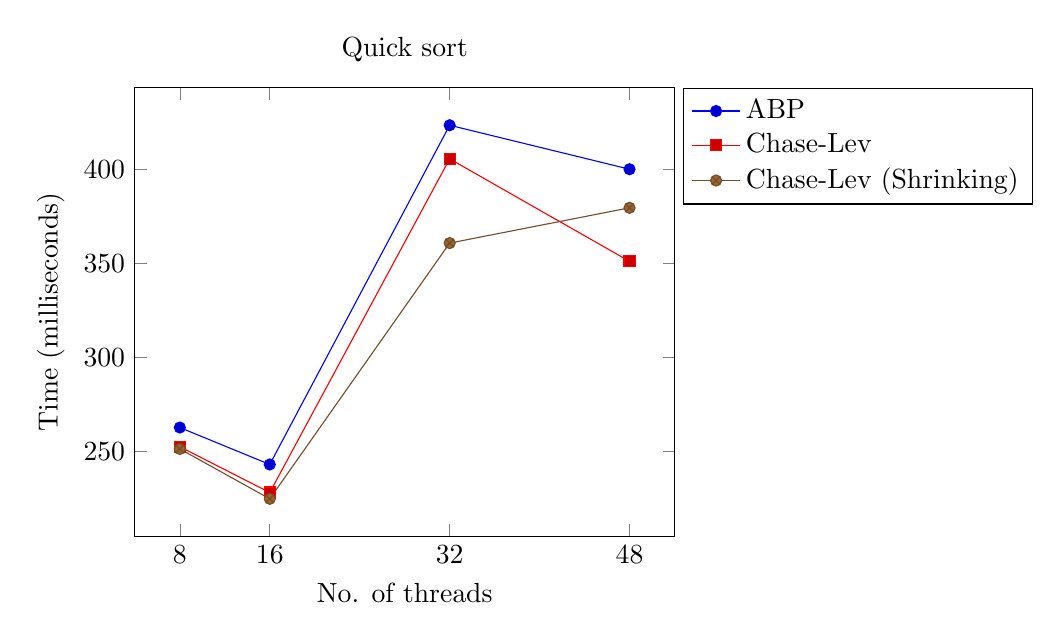
\begin{tikzpicture}
\begin{axis}[
  title={Quick sort},
  xlabel={No. of threads},
  ylabel={Time (milliseconds)},
  xtick={8,16,32,48},
  legend style={at={(1.34,1)}, anchor=north,legend columns=1},
  legend cell align=left
  ]
\addplot+[sharp plot] coordinates % ABP
{(8,262.86) (16,243.2) (32,423.68) (48, 400.28)};
\addplot+[sharp plot] coordinates % Chase-Lev
{(8,252.67) (16,228.27) (32,405.8) (48, 351.26)};
\addplot+[sharp plot] coordinates % Chase-Lev (Shrinking
{(8,251.47) (16,224.93) (32,360.98) (48, 379.75)};
\legend{ABP, Chase-Lev, Chase-Lev (Shrinking)}
\end{axis}
\end{tikzpicture}
\end{figure}

\begin{figure}
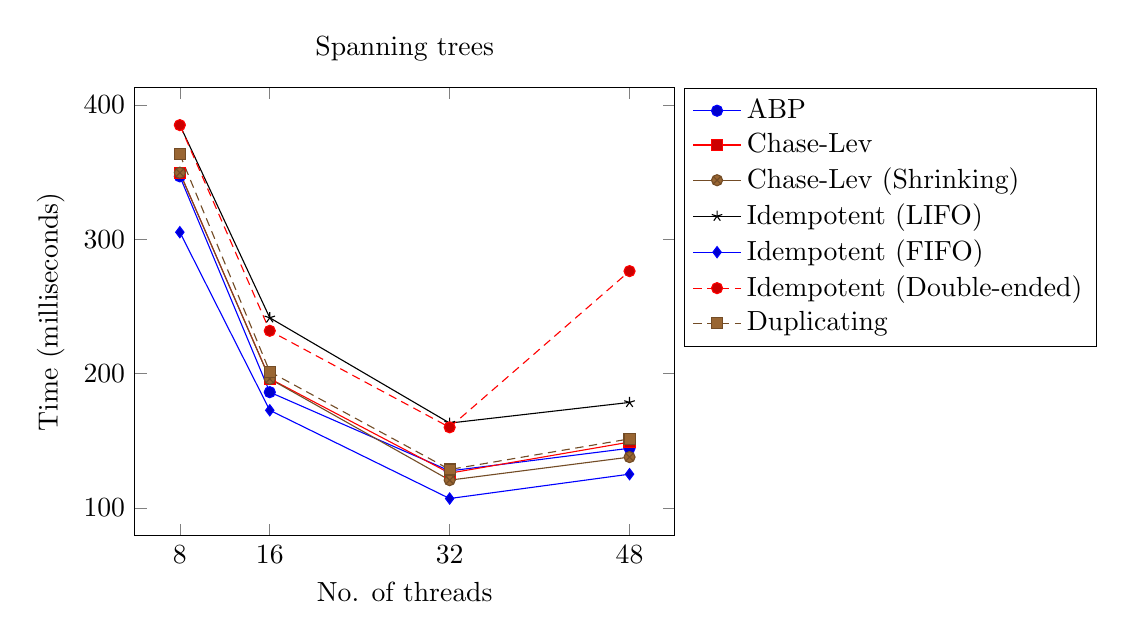
\begin{tikzpicture}
\begin{axis}[
  title={Spanning trees},
  xlabel={No. of threads},
  ylabel={Time (milliseconds)},
  xtick={8,16,32,48},
  legend style={at={(1.4,1)}, anchor=north,legend columns=1},
  legend cell align=left
  ]
\addplot+[sharp plot] coordinates % ABP
{(8,346.81) (16,186.23) (32,127.63) (48, 144.5)};
\addplot+[sharp plot] coordinates % Chase-Lev
{(8,349.47) (16,196.33) (32,125.96) (48, 149.09)};
\addplot+[sharp plot] coordinates % Chase-Lev (Shrinking)
{(8,349.53) (16,196.08) (32,120.76) (48, 137.92)};
\addplot+[sharp plot] coordinates % Idempotent (LIFO)
{(8,385.08) (16,241.58) (32,163.23) (48, 178.6)};
\addplot+[sharp plot] coordinates % Idempotent (FIFO)
{(8,305.27) (16,172.76) (32,107.09) (48, 125.22)};
\addplot+[sharp plot] coordinates % Idempotent (Double-ended)
{(8,384.94) (16,231.89) (32,160.05) (48, 276.3)};
\addplot+[sharp plot] coordinates % Duplicating
{(8,363.15) (16,201.47) (32,128.69) (48, 151.47)};
\legend{ABP, Chase-Lev, Chase-Lev (Shrinking), Idempotent (LIFO), Idempotent (FIFO),
        Idempotent (Double-ended), Duplicating}
\end{axis}
\end{tikzpicture}
\end{figure}

\begin{figure}
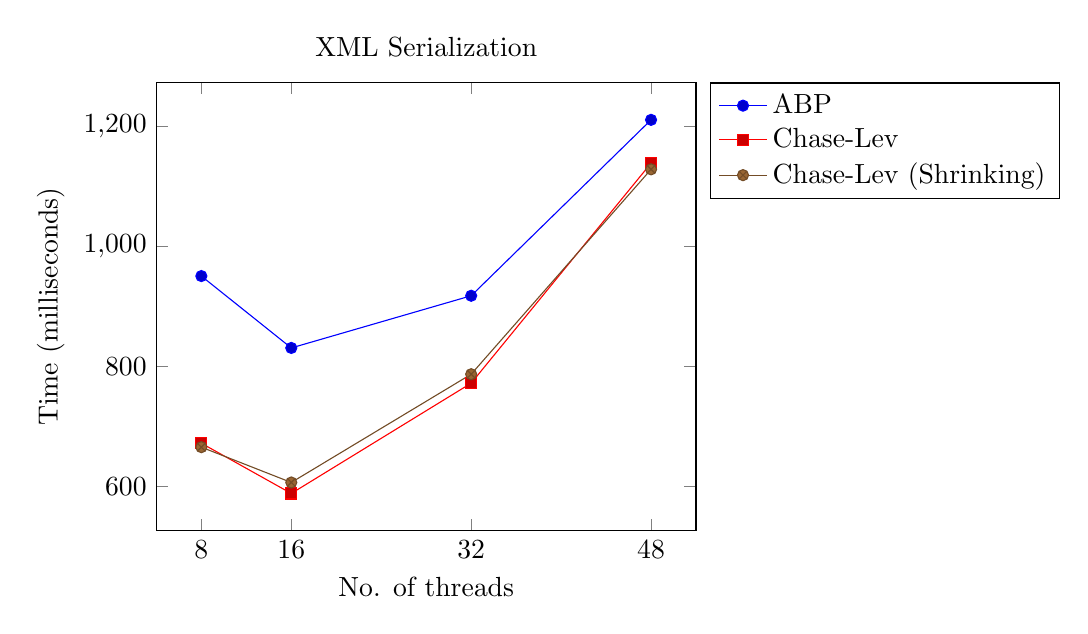
\begin{tikzpicture}
\begin{axis}[
  title={XML Serialization},
  xlabel={No. of threads},
  ylabel={Time (milliseconds)},
  xtick={8,16,32,48},
  legend style={at={(1.35,1)}, anchor=north,legend columns=1},
  legend cell align=left
  ]
\addplot+[sharp plot] coordinates % ABP
{(8,950.29) (16,830.74) (32,917.55) (48, 1210.11)};
\addplot+[sharp plot] coordinates % Chase-Lev
{(8,672.29) (16,588.71) (32,772.17) (48, 1138.10)};
\addplot+[sharp plot] coordinates % Chase-Lev (Shrinking
{(8,665.72) (16,606.98) (32,787.06) (48, 1127.79)};
\legend{ABP, Chase-Lev, Chase-Lev (Shrinking)}
\end{axis}
\end{tikzpicture}
\end{figure}

\begin{figure}
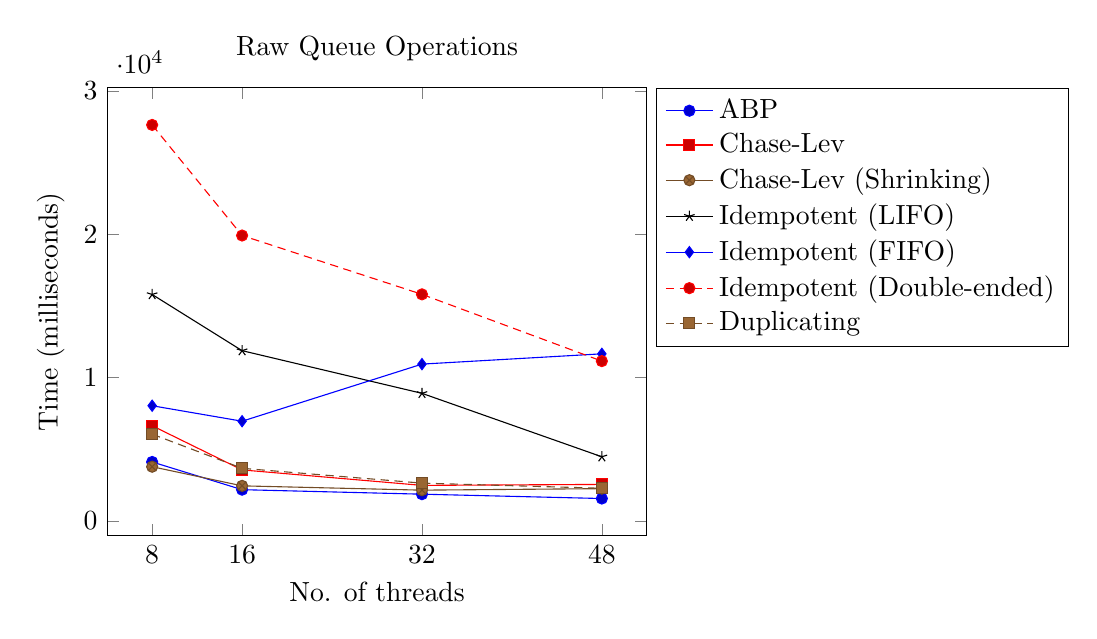
\begin{tikzpicture}
\begin{axis}[
  title={Raw Queue Operations},
  xlabel={No. of threads},
  ylabel={Time (milliseconds)},
  xtick={8,16,32,48},
  legend style={at={(1.4,1)}, anchor=north,legend columns=1},
  legend cell align=left
  ]
\addplot+[sharp plot] coordinates % ABP
{(8,4120.79) (16,2188.83) (32,1874.62) (48, 1572.27)};
\addplot+[sharp plot] coordinates % Chase-Lev
{(8,6646.03) (16,3566.86) (32,2488.21) (48, 2556.13)};
\addplot+[sharp plot] coordinates % Chase-Lev (Shrinking)
{(8,3788.95) (16,2455.44) (32,2155.72) (48, 2261.03)};
\addplot+[sharp plot] coordinates % Idempotent (LIFO)
{(8,15797.32) (16,11881.41) (32,8905.86) (48, 4482.83)};
\addplot+[sharp plot] coordinates % Idempotent (FIFO)
{(8,8041.34) (16,6962.21) (32,10943.90) (48, 11661.40)};
\addplot+[sharp plot] coordinates % Idempotent (Double-ended)
{(8,27620.75) (16,19909.84) (32,15807.66) (48, 11152.57)};
\addplot+[sharp plot] coordinates % Duplicating
{(8,6061.63) (16,3679.41) (32,2645.78) (48, 2286.77)};
\legend{ABP, Chase-Lev, Chase-Lev (Shrinking), Idempotent (LIFO), Idempotent (FIFO),
        Idempotent (Double-ended), Duplicating}
\end{axis}
\end{tikzpicture}
\end{figure}